%%%%%%%%%%%%%%%%%%%%%%%%%%%%%%%%%%%%%%%%%
% Cleese Assignment (For Students)
% LaTeX Template
% Version 2.0 (27/5/2018)
%
% This template originates from:
% http://www.LaTeXTemplates.com
%
% Author:
% Vel (vel@LaTeXTemplates.com)
%
% License:
% CC BY-NC-SA 3.0 (http://creativecommons.org/licenses/by-nc-sa/3.0/)
% 
%%%%%%%%%%%%%%%%%%%%%%%%%%%%%%%%%%%%%%%%%

%----------------------------------------------------------------------------------------
%	PACKAGES AND OTHER DOCUMENT CONFIGURATIONS
%----------------------------------------------------------------------------------------
\RequirePackage[2020-02-02]{latexrelease}
\documentclass[11pt]{article}
\usepackage{float}
\usepackage{tikz}
\usepackage{listings}
\usepackage{color} %red, green, blue, yellow, cyan, magenta, black, white
\definecolor{mygreen}{RGB}{28,172,0} % color values Red, Green, Blue
\definecolor{mylilas}{RGB}{170,55,241}
\usepackage{amsmath, amssymb}
\DeclareMathOperator{\sinc}{sinc}
\DeclareMathOperator{\sgn}{sgn}
\usepackage[american]{circuitikz}

%%%%%%%%%%%%%%%%%%%%%%%%%%%%%%%%%%%%%%%%%
% Cleese Assignment
% Structure Specification File
% Version 1.0 (27/5/2018)
%
% This template originates from:
% http://www.LaTeXTemplates.com
%
% Author:
% Vel (vel@LaTeXTemplates.com)
%
% License:
% CC BY-NC-SA 3.0 (http://creativecommons.org/licenses/by-nc-sa/3.0/)
% 
%%%%%%%%%%%%%%%%%%%%%%%%%%%%%%%%%%%%%%%%%

%----------------------------------------------------------------------------------------
%	PACKAGES AND OTHER DOCUMENT CONFIGURATIONS
%----------------------------------------------------------------------------------------

\usepackage{lastpage} % Required to determine the last page number for the footer

\usepackage{graphicx} % Required to insert images

\setlength\parindent{0pt} % Removes all indentation from paragraphs

\usepackage[most]{tcolorbox} % Required for boxes that split across pages

\usepackage{booktabs} % Required for better horizontal rules in tables

\usepackage{listings} % Required for insertion of code

\usepackage{etoolbox} % Required for if statements

%----------------------------------------------------------------------------------------
%	MARGINS
%----------------------------------------------------------------------------------------

\usepackage{geometry} % Required for adjusting page dimensions and margins

\geometry{
	paper=a4paper, % Change to letterpaper for US letter
	top=3cm, % Top margin
	bottom=3cm, % Bottom margin
	left=2.5cm, % Left margin
	right=2.5cm, % Right margin
	headheight=14pt, % Header height
	footskip=1.4cm, % Space from the bottom margin to the baseline of the footer
	headsep=1.2cm, % Space from the top margin to the baseline of the header
	%showframe, % Uncomment to show how the type block is set on the page
}

%----------------------------------------------------------------------------------------
%	FONT
%----------------------------------------------------------------------------------------

\usepackage[utf8]{inputenc} % Required for inputting international characters
\usepackage[T1]{fontenc} % Output font encoding for international characters

\usepackage[sfdefault,light]{roboto} % Use the Roboto font

%----------------------------------------------------------------------------------------
%	HEADERS AND FOOTERS
%----------------------------------------------------------------------------------------

\usepackage{fancyhdr} % Required for customising headers and footers

\pagestyle{fancy} % Enable custom headers and footers

\lhead{\small\assignmentClass\ifdef{\assignmentClassInstructor}{\ (\assignmentClassInstructor):}{}\ \assignmentTitle} % Left header; output the instructor in brackets if one was set
\chead{} % Centre header
\rhead{\small\ifdef{\assignmentAuthorName}{\assignmentAuthorName}{\ifdef{\assignmentDueDate}{Due\ \assignmentDueDate}{}}} % Right header; output the author name if one was set, otherwise the due date if that was set

\lfoot{} % Left footer
\cfoot{\small Page\ \thepage\ of\ \pageref{LastPage}} % Centre footer
\rfoot{} % Right footer

\renewcommand\headrulewidth{0.5pt} % Thickness of the header rule

%----------------------------------------------------------------------------------------
%	MODIFY SECTION STYLES
%----------------------------------------------------------------------------------------

\usepackage{titlesec} % Required for modifying sections

%------------------------------------------------
% Section

\titleformat
{\section} % Section type being modified
[block] % Shape type, can be: hang, block, display, runin, leftmargin, rightmargin, drop, wrap, frame
{\Large\bfseries} % Format of the whole section
{\assignmentQuestionName~\thesection} % Format of the section label
{6pt} % Space between the title and label
{} % Code before the label

\titlespacing{\section}{0pt}{0.5\baselineskip}{0.5\baselineskip} % Spacing around section titles, the order is: left, before and after

%------------------------------------------------
% Subsection

\titleformat
{\subsection} % Section type being modified
[block] % Shape type, can be: hang, block, display, runin, leftmargin, rightmargin, drop, wrap, frame
{\itshape} % Format of the whole section
{(\alph{subsection})} % Format of the section label
{4pt} % Space between the title and label
{} % Code before the label

\titlespacing{\subsection}{0pt}{0.5\baselineskip}{0.5\baselineskip} % Spacing around section titles, the order is: left, before and after

\renewcommand\thesubsection{(\alph{subsection})}

%----------------------------------------------------------------------------------------
%	CUSTOM QUESTION COMMANDS/ENVIRONMENTS
%----------------------------------------------------------------------------------------

% Environment to be used for each question in the assignment
\newenvironment{question}{
	\vspace{0.5\baselineskip} % Whitespace before the question
	\section{} % Blank section title (e.g. just Question 2)
	\lfoot{\small\itshape\assignmentQuestionName~\thesection~continued on next page\ldots} % Set the left footer to state the question continues on the next page, this is reset to nothing if it doesn't (below)
}{
	\lfoot{} % Reset the left footer to nothing if the current question does not continue on the next page
}

%------------------------------------------------

% Environment for subquestions, takes 1 argument - the name of the section
\newenvironment{subquestion}[1]{
	\subsection{#1}
}{
}

%------------------------------------------------

% Command to print a question sentence
\newcommand{\questiontext}[1]{
	\textbf{#1}
	\vspace{0.5\baselineskip} % Whitespace afterwards
}

%------------------------------------------------

% Command to print a box that breaks across pages with the question answer
\newcommand{\answer}[1]{
	\begin{tcolorbox}[breakable, enhanced]
		#1
	\end{tcolorbox}
}

%------------------------------------------------

% Command to print a box that breaks across pages with the space for a student to answer
\newcommand{\answerbox}[1]{
	\begin{tcolorbox}[breakable, enhanced]
		\vphantom{L}\vspace{\numexpr #1-1\relax\baselineskip} % \vphantom{L} to provide a typesetting strut with a height for the line, \numexpr to subtract user input by 1 to make it 0-based as this command is
	\end{tcolorbox}
}

%------------------------------------------------

% Command to print an assignment section title to split an assignment into major parts
\newcommand{\assignmentSection}[1]{
	{
		\centering % Centre the section title
		\vspace{2\baselineskip} % Whitespace before the entire section title
		
		\rule{0.8\textwidth}{0.5pt} % Horizontal rule
		
		\vspace{0.75\baselineskip} % Whitespace before the section title
		{\LARGE \MakeUppercase{#1}} % Section title, forced to be uppercase
		
		\rule{0.8\textwidth}{0.5pt} % Horizontal rule
		
		\vspace{\baselineskip} % Whitespace after the entire section title
	}
}

%----------------------------------------------------------------------------------------
%	TITLE PAGE
%----------------------------------------------------------------------------------------

\author{\textbf{\assignmentAuthorName}} % Set the default title page author field
\date{} % Don't use the default title page date field

\title{
	\thispagestyle{empty} % Suppress headers and footers
	\vspace{0.2\textheight} % Whitespace before the title
	\textbf{\assignmentClass:\ \assignmentTitle}\\[-4pt]
	\ifdef{\assignmentDueDate}{{\small Due\ on\ \assignmentDueDate}\\}{} % If a due date is supplied, output it
	\ifdef{\assignmentClassInstructor}{{\large \textit{\assignmentClassInstructor}}}{} % If an instructor is supplied, output it
	\vspace{0.32\textheight} % Whitespace before the author name
}
 % Include the file specifying the document structure and custom commands

%----------------------------------------------------------------------------------------
%	ASSIGNMENT INFORMATION
%----------------------------------------------------------------------------------------

% Required
\newcommand{\assignmentQuestionName}{Task} % The word to be used as a prefix to question numbers; example alternatives: Problem, Exercise
\newcommand{\assignmentClass}{Electrical Circuits (Taught by Mohammad Hadi)\\Final Project (Due on DDD.,\ mmm.\ dd,\ yyyy)} % Course (Lecturer)\\Assignment (Due date)
\newcommand{\assignmentTitle}{} % Assignment title or name
\newcommand{\assignmentAuthorName}{Student Name\\Student Number} % Student name\\Student number
%----------------------------------------------------------------------------------------

\begin{document}
\lstset{language=Python,%
	basicstyle={\scriptsize},
	breaklines=true,%
	morekeywords={matlab2tikz},
	keywordstyle=\color{blue},%
	morekeywords=[2]{1}, keywordstyle=[2]{\color{black}},
	identifierstyle=\color{black},%
	stringstyle=\color{mylilas},
	commentstyle=\color{mygreen},%
	showstringspaces=false,%without this there will be a symbol in the places where there is a space
	numbers=left,%
	numberstyle={\tiny \color{black}},% size of the numbers
	numbersep=5pt, % this defines how far the numbers are from the text
	emph=[1]{break},emphstyle=[1]\color{red}, %some words to emphasise
	%emph=[2]{word1,word2}, emphstyle=[2]{style},    
}
%----------------------------------------------------------------------------------------
%	TITLE PAGE
%----------------------------------------------------------------------------------------
\textbf{Feel free to do one of the following tasks as your final project. I personally prefer the engineering task 
although it needs to have access to an oscilloscope. In my view, you become familiar with many practical points while doing the engineering task. }

\assignmentSection{Engineering Task}

%----------------------------------------------------------------------------------------
%	Task 1
%----------------------------------------------------------------------------------------

\begin{question}

\questiontext{Stereo audio has two audio signals designed for two separate audio channels, which creates a perception of space. If you have a stereo headphone, each audio signal is played separately on a speaker. The two audio signals can be injected to an oscilloscope in xy mode to create a Lissajous curve.}

\begin{figure}[H] 
\begin{center}
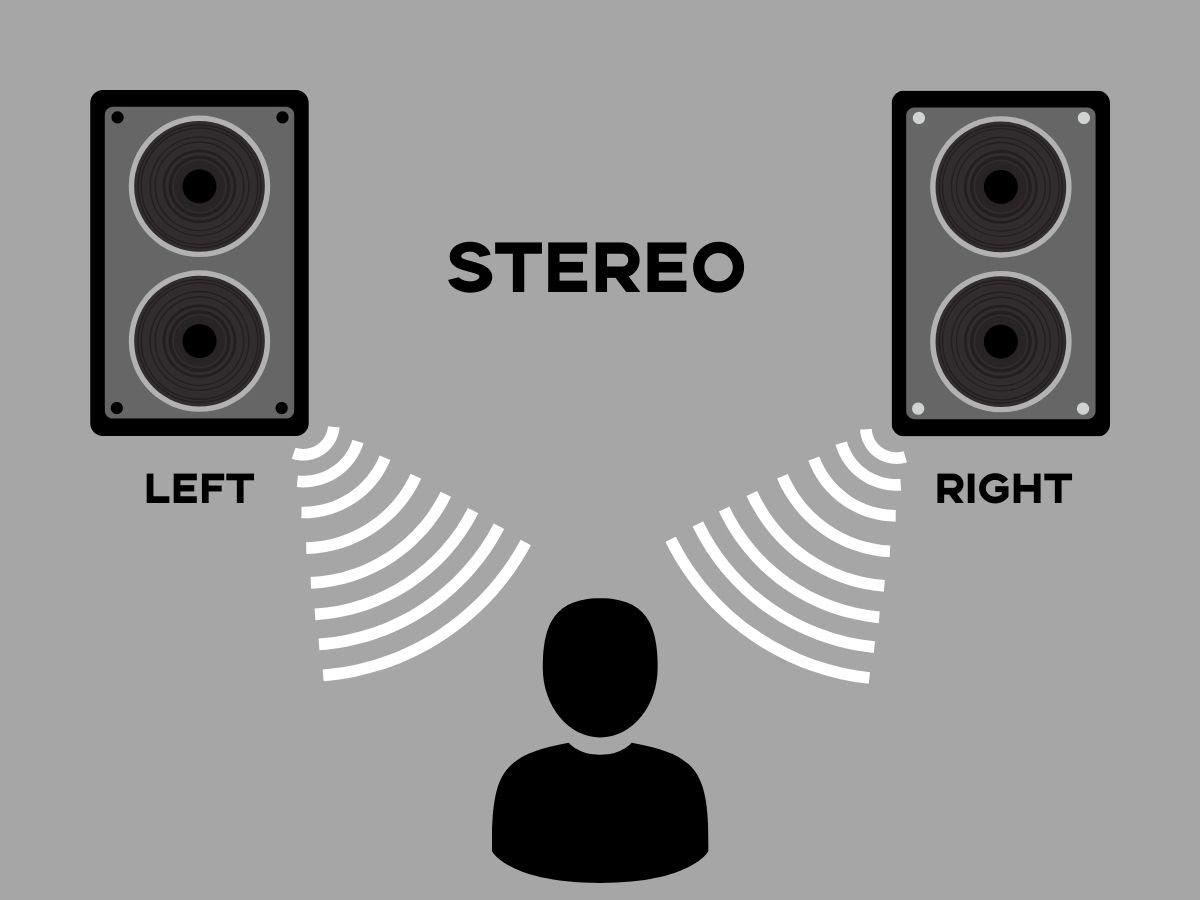
\includegraphics[scale=0.2]{Fig/stereo.jpg}
\caption{\label{fig:stereo} Stereo audio on speakers.}
\end{center}
\end{figure}  

%--------------------------------------------
\begin{subquestion}{Write a MATLAB/Python code to create suitable stereo audio such that the corresponding Lissajous curve on an oscilloscope looks like a heart shape. Connect the audio output of your laptop using a stereo audio jack to the channels of an oscilloscope and see the heart-shaped Lissajous curve. } 
\answer{
	If we want to use python, we must use "sounddevice", "numpy" and "matplotlib.pyplot" library. In case of making heart once the program is executed, it will generate a sine wave for X axis and a combination of four cosine waves for Y axis with a frequency of 44100 Hz and duration of 10 seconds. The signal will be outputted through the specified audio output device, which should be connected to your oscilloscope via the AUX cable.\\
	
	\textbf{Heart:}
	\lstinputlisting{Fig/Heart.py}
	\begin{figure}[H]
		\centering
		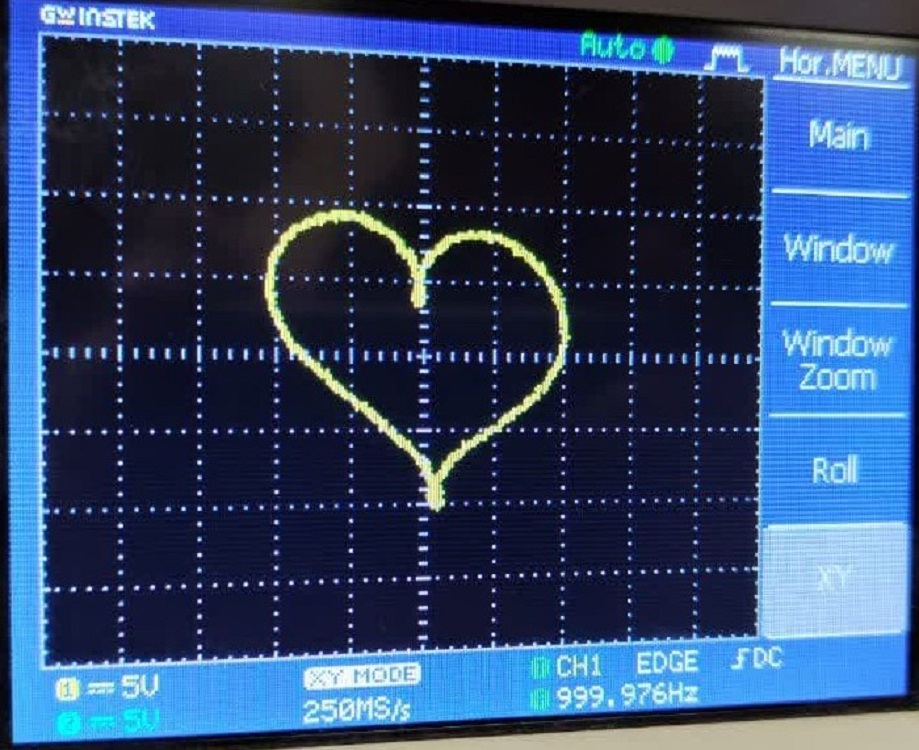
\includegraphics[scale=0.4,angle=0]{Fig/Heart.jpg}
		\caption{Heart in xy mode of oscilloscope.} \label{fig:cir2}
	\end{figure}
}
\end{subquestion}
%--------------------------------------------
\begin{subquestion}{Extend your code such that common geometric shapes like circle, ellipse, square, and so on appear as a Lissajous curve on the oscilloscope.} 
\answer{
	In case of making circle once the program is executed, it will generate a cosine wave for X axis and sine waves for Y axis with a frequency of 44100 Hz and duration of 10 seconds.
	\textbf{Circle:}\\
	\lstinputlisting{Fig/Circle.py}
	\begin{figure}[H]
		\centering
		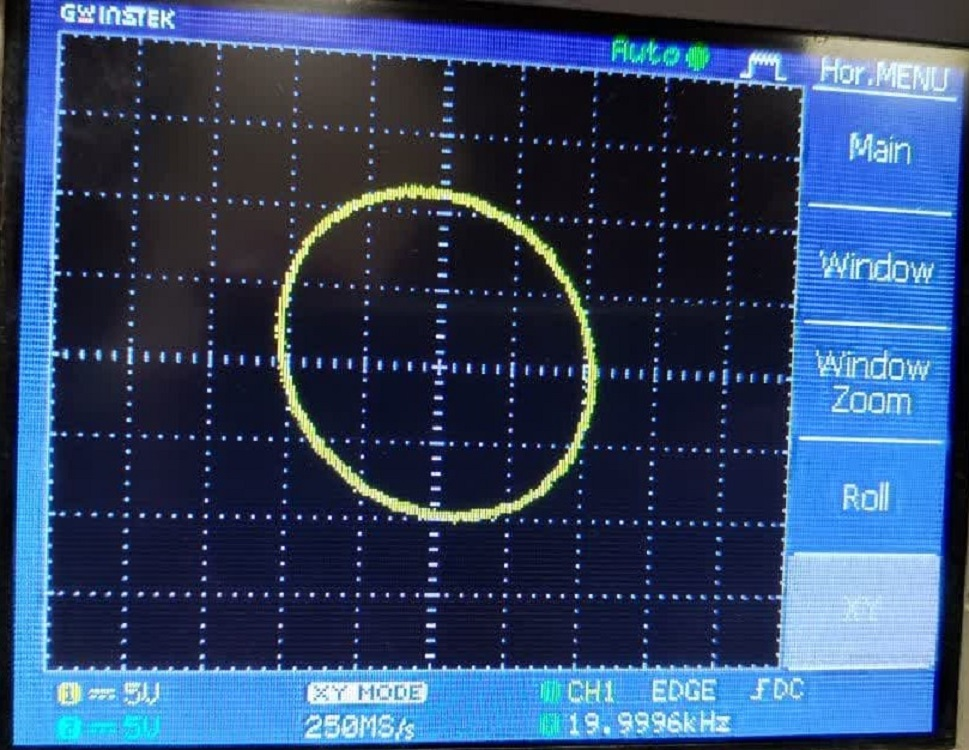
\includegraphics[scale=0.4,angle=0]{Fig/Circle.jpg}
		\caption{Circle in xy mode of oscilloscope.} \label{fig:cir2}
	\end{figure}
	In case of making Ellipse once the program is executed, it will generate a cosine wave for X axis and sine waves for Y axis with a frequency of 44100 Hz and duration of 10 seconds.
	\textbf{Ellipse:}\\
	\lstinputlisting{Fig/Ellipse.py}
	\begin{figure}[H]
		\centering
		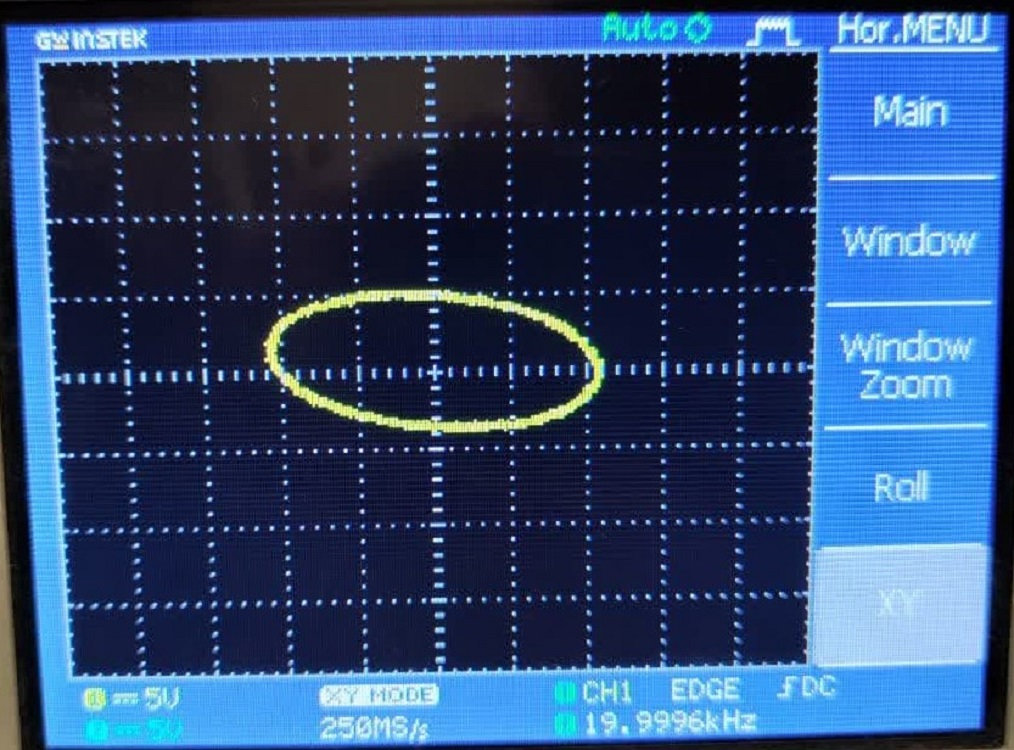
\includegraphics[scale=0.4,angle=0]{Fig/Ellipse.jpg}
		\caption{Ellipse in xy mode of oscilloscope.} \label{fig:cir2}
	\end{figure}
	\textbf{Square:}\\
	\lstinputlisting{Fig/Square.py}
	\textbf{Diamond:}\\
	\lstinputlisting{Fig/Diamond.py}
	\begin{figure}[H]
		\centering
		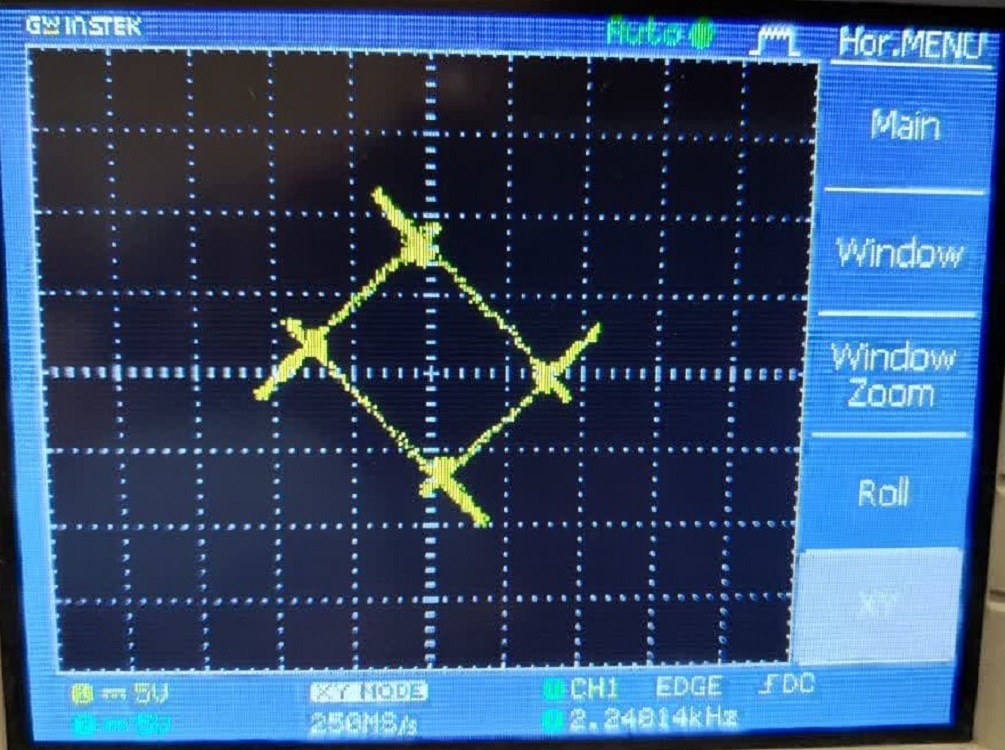
\includegraphics[scale=0.4,angle=0]{Fig/Diamond.jpg}
		\caption{Diamond in xy mode of oscilloscope.} \label{fig:cir2}
	\end{figure}
	\textbf{Animated Circle:}\\
	\lstinputlisting{Fig/AnimatedCircle.py}
}
\end{subquestion}

%--------------------------------------------
\begin{subquestion}{Prepare a short report and describe your work concisely. Use suitable figures or equations to  better describe different parts of your code and to make your report more readable and understandable. Take a short video of yourself demonstrating the creation of the desired Lissajous curves. 
} 
\answer{}
\end{subquestion}


%--------------------------------------------
\begin{subquestion}{\textbf{Bonus!} Create a GUI for your code such that the desired curve is taken as a two-dimensional function $f(x,y)=0$ and its corresponding Lissajous curve appears on the oscilloscope.
} 
\answer{}
\end{subquestion}

%--------------------------------------------
\begin{subquestion}{\textbf{Bonus!} Write your report in \LaTeX.
} 
\end{subquestion}

\end{question}

\end{document}
